\documentclass[12pt, letterpaper, oneside]{book}
%\documentclass[12pt, letterpaper]{book}

\usepackage[spanish,es-tabla]{babel}
\usepackage[utf8x]{inputenc}
\usepackage{mathtools}
\usepackage{microtype}
\usepackage{emptypage}
\usepackage{usmtesis}
\usepackage{url}
\usepackage{caption}
\usepackage{amsmath}
\usepackage{listings}
%\usepackage{graphicx}
\usepackage{subcaption}
\usepackage{cite}
\usepackage{rotating}
\usepackage{amsfonts}
\usepackage{hyperref}
\usepackage{algorithm}
\usepackage{algorithmic}

\usepackage{tikz}
\usetikzlibrary{babel,arrows.meta,shapes,arrows}

%\usepackage{layout} %debug only

\RequirePackage{fancyhdr}
\newcommand{\hsp}[1][20]{\hspace{#1pt}}
\fancyhf{}
\fancypagestyle{plain}{%
	\fancyhf{} 
	\fancyhead[L]{\scriptsize \rightmark}
	\fancyhead[R]{\scriptsize \leftmark}
	\fancyfoot[R]{\bfseries \thepage}
	\fancyfoot[L]{Departamento de Informática. UTFSM.}
	\renewcommand{\headrulewidth}{0.1pt}
	\renewcommand{\footrulewidth}{0.1pt}
}
%\setlength{\footheight}{110pt} 

%macros
\renewcommand{\tt}[1]{\texttt{#1}}
\renewcommand{\bf}[1]{\textbf{#1}}
\newcommand{\etal}{\emph{et al.}}

\begin{document}
\frontmatter
\thispagestyle{empty}
%!TEX root = main.tex

\begin{center}
  \begin{spacing}{1}
    {\large UNIVERSIDAD TÉCNICA FEDERICO SANTA MARÍA}\\
    DEPARTAMENTO DE INFORMÁTICA\\
    VALPARAÍSO - CHILE
  \end{spacing}

  \vspace{12mm}
  
\includegraphics[height=50mm]{figures/usm_logo.png}
  \vspace{15mm}

  \begin{spacing}{1.5} 
    \textbf{\large \emph{Particle Swarm Optimization} para el ajuste de modelos
      probabilísticos a datos del viento en Valparaíso}\\
    %\textbf{\large asd}\\
  \end{spacing}

  \vspace{20mm}
  \textbf{\large ALONSO JAVIER SANDOVAL ACEVEDO}
  \vspace{12mm}

  \begin{spacing}{1.25} 
    MEMORIA PARA OPTAR AL TÍTULO DE\\
    INGENIERO CIVIL EN INFORMÁTICA
    %PRIMER AVANCE DE MEMORIA
  \end{spacing}

  \vspace{15mm}
  \begin{table}[h]
    \begin{center}
      \begin{tabular}{ l c l }
        PROFESOR GUÍA & : & MARÍA CRISTINA RIFF.\\
        PROFESOR CORREFERENTE & : & X. X.\\
      \end{tabular}
    \end{center}
  \end{table}

  \vfill
  \large JULIO 2016
\end{center}

\newpage

%debug
%\layout
%\newpage

%% Hack para el abstract corregir si se puede.
%\chapter*{ }
%\vspace{-3cm}
%\section*{Abstact} \chaptermark{Abstract}
%\section*{Resumen}

\begin{spacing}{1}
\tableofcontents \chaptermark{Tabla de contenidos}
\listoffigures
%\listoftables
\end{spacing}

\mainmatter

%!TEX root = main.tex

\chapter{Introducción}

\section{Identificación del problema}
El viento es uno de los fenómenos metereológicos más comunes de las zonas costeras de Valparaíso. Sus características afectan distintos aspectos del entorno que influyen en nuestras vidas, como las condiciones del clima, la sensación térmica, algunos desastres naturales, entre otros. Esto atrae el interés de los especialistas, fomentando la investigación para lograr controlar, en cierta medida, las distintas variables que condicionan su comportamiento, de manera de poder predecir los fenómenos subyacentes a este. Más aún, el viento es ampliamente conocido por ser una fuente renovable y poco contaminante de energía, comunmente llamada energía eólica, lo que hace aún más interesante y necesario el estudio de este fenómeno metereológico.\\
En los últimos años, tanto el gobierno de Chile como la ciudadanía, han mostrado un creciente interés en las fuentes de energías renovables y con mínimo impacto ambiental, por lo que distintos proyectos en la matería han sido llevados a cabo, desde estudios de factibilidad y recopilación de datos hasta el emplazamiento de las primeras centrales de fuentes de energía límpia. El año 2014, el ministerio de energía publicó un extenso reporte acerca de la situación actual del país en materias de energías renovables, en donde se pueden ver distintas proyecciones y estimaciones de implementación de posibles plantas de generación a lo largo del país. \cite{minenergia14}\\
Cualquiera sea el estudio de las condiciones climáticas del viento para predecir su potencial energético, existen dos variables fundamentales ha considerar para obtener estas predicciones: la velocidad y la dirección del viento. Actualmente, estos datos están disponibles y son obtenidos por diversos centros metereológicos a lo largo del país, en partícular, el servicio metereológico de la Armada de Chile, que cuenta con el equipo necesario para registrar el comportamiento del viento al lo largo de las distintas épocas del año y en diferentes zonas de Chile.\\
Si bien la obtención de los datos es un paso, para poder obtener información o conocimiento relevante sobre estos (algo más que un promedio, por ejemplo), es necesario generar modelos que permitan ``explicar'' la distribución de datos y de cierta forma predecir el comportamiento futuro del viento. En la literatura, son ampliamente aceptadas la distribución de \emph{Weibull} para modelar el conjunto datos de velocidad y la distribución de Von Mises para el modelo de la dirección del viento. Ambas distribuciones probabilísticas requieren de la determinación de parámetros para que el modelo se ajuste a los datos obtenidos. Comunmente, se utilizan métodos númericos para la determinación de estos parámetros, sin embargo, estudios recientes han demostrado que la utilización de algorítmos basados en la metaheurística \emph{Particle Swarm Optimization} mejoran los parámetros obtenidos por los métodos tradicionales y por ende la aproximación del modelo al comportamiento real.\\ 

\section{Objetivos}
Aplicar métodos actuales de optimización basados en la metaheurística \emph{Particle Swarm Optimization} para el ajuste de modelos probabilísticos de dirección y velocidad del viento a los datos recopilados del viento en Valparaíso, con el fin de presentar resultados que permitan inferir información precisa acerca de las condiciones de la región para la generación de energía eólica y otras potenciales aplicaciones.

\subsection{Objetivos específicos}
\begin{enumerate}
    \item Implementar un algoritmo basado en \emph{Particle Optimization Sworm} para \textbf{encontrar} los parámetros de un modelo probabilístico que se ajusten a los datos de la velocidad del viento en Valparaíso. 
    \item Implementar un algoritmo basado en \emph{Particle Optimization Sworm} para \textbf{optimizar} los parámetros de un modelo probabilístico que se ajusten a los datos de la dirección del viento en Valparaíso.
    \item Evaluar los modelos sobre los datos del viento para validar la propuesta realizada.
\end{enumerate}


%!TEX root = main.tex

\chapter{Estado del arte}
\section{Particle Swarm Optimization}
Como se introduce en el artículo de Kaveh \cite{Psoexplain14}, el algoritmo \emph{Particle Swarm Optimization} es una meta-heurística inspirada en las observaciones de la naturaleza acerca del comportamiento social de poblaciones de enjambres. Esta abstracción está basada, por ejemplo, en las gaviotas, las cuales suelen moverse en grupos, conocidos como bandadas, cerca del mar en búsqueda de zonas donde hayan alimento (peces). El método simula la conducta de los individuos a través de partículas que se mueven dentro de un espacio (de búsqueda), siendo estas afectadas por factores individuales (conocimiento propio) y colectivos (conocimiento del enjambre), los cuales dirigen el movimiento de estos grupos a ciertas zonas las que son determinadas por una función objetivo (\emph{fitness function}).\\
Para cada partícula su vector posición  $\vec{x}$ representa una solución candidata, la cual varía dentro del espacio de búsqueda a velocidad $\vec{v}$. Después de varias iteraciones, el enjambre o conjunto de partículas, se irá concentrando en aquellas zonas donde la posición obtenga mejores valores para la función objetivo.
\\El modelo clásico presentado por Kennedy y Eberhart\cite{Kennedy95}, describe la variación de la velocidad y de la posición de las partículas como se presenta a continuación:
\begin{align}
    v_{i,j}^{k+1} &= v_{i,j}^{k} + c_{1}r_{1}(xbest_{i,j}^k - x_{i,j}^k) + c_{2}r_{2}(xgbest_{j}^{k} - x_{i,j}^k) \\
    x_{i,j}^{k+1} &= x_{i,j}^{k} + v_{i,j}^{k+1}
\end{align}    
Como se explica en Kaveh \cite{Psoexplain14} $x_{i,j}^{k}$ y $v_{i,j}^{k}$ son la $j$-ésima componente de la posición y la velocidad de la partícula $i$ respectivamente en la iteración o tiempo $k$, $r_{1}$ y $r_{2}$ son número aleatorios uniformes que varían de 0 a 1, $xbest_i$ y $xgbest$ representan las mejores soluciones alcanzadas por la partícula y por el enjambre respectivamente, $c_1$ y $c_2$ son parámetros que representan la confianza en la solución individual de la partícula (parámetro cognitivo) y la incidencia del aspecto colectivo o solución global (parámetro social), respectivamente. Un esquema de la interacción de estos componentes se aprecia en la figura \ref{fig:move_part}\\
\begin{figure}[h!]
    \centering    
    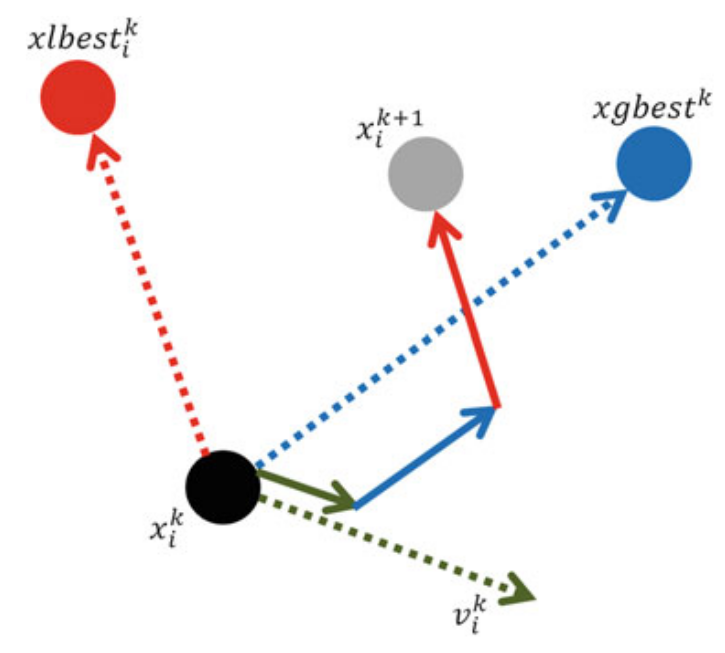
\includegraphics[height=50mm]{figures/move_particle.png} 
    \caption{Movimiento de una partícula}
    \vspace{-.25cm} 
    \caption*{Creado por Kaveh\cite{Psoexplain14}.}
    \label{fig:move_part}
\end{figure}
El modelo clásico presentado tiene ciertas complicaciones en la forma en que se actualiza la velocidad, una de ellas es la incidencia de la velocidad previa en una partícula, por lo que a modo de balancear esta variable, se añade un factor que escala esta velocidad, dado que como se explica en Kaveh \cite{Psoexplain14}, si la velocidad previa se elimina, las partículas quedan atrapadas en una región local, pero si se le da demasiado peso, converge rápidamente a un óptimo conocido. Por esto, la forma del PSO base actual, tiene un parámetro $w$, que representa la incidencia de la velocidad previa (factor de inercia). Por lo tanto, ahora se tiene que la partícula actualiza su velocidad de la siguiente forma: 
\begin{align}\label{eq:PSO}
    v_{i,j}^{k+1} &= wv_{i,j}^{k} + c_{1}r_{1}(xbest_{i,j}^k - x_{i,j}^k) + c_{2}r_{2}(xgbest_{j}^{k} - x_{i,j}^k)\\
    x_{i,j}^{k+1} &= x_{i,j}^{k} + v_{i,j}^{k+1}
\end{align}    
Donde $w$ es el factor conocido como ``inercia'' de la partícula, y regula la incidencia de la velocidad previa en la actual.\\
Finalmente, en el trabajo inicialmente citado, también se puede ver una revisión completa del estado del arte del método \emph{Particle Swarm Optimization} en términos de diseño, donde se expone las distintas modificaciones y alternativas propuestas por la literatura que pretenden mejorar aspectos como:
\begin{enumerate}
    \item  Configuración de parámetros (inercia, cognitivo, social, aleatorios).
    \item  Problemas asociados a la convergencia prematura.
    \item  Estructura de algoritmo o topologías que modifican la comunicación entre partículas (o la incidencia de las soluciones globales y particulares).
    \item  Sesgos en la búsqueda por la forma de la región o por la interacción de las partículas (operadores de combinación como el promedio, que tienden a centrar la búsqueda en determinada región).
    \item  Algoritmos híbridos con PSO.
    \item  Versión discreta del PSO. 
\end{enumerate}  

\section{Velocidad del viento}
\subsection{Distribución de Weibull}
Dado un conjunto de datos de velocidad obtenidos de la medición del viento, se puede crear un histograma que represente la frecuencia de estos datos. A partir de esto, es posible generar un modelo probabilístico que explique el comportamiento de las velocidades del viento medido, ajustándose a los datos recolectados. Dicho modelo comúnmente se basa en la distribución de Weibull, la cual es ampliamente aceptada por la comunidad dedicada al estudio meteorológico, tal y como se menciona en el trabajo de Carneiro et al. \cite{Carneiro15}, Kongnam et al. \cite{Kongnam15} y Dabbaghiyan et al.\cite{Dabbaghiyan15}. En particular, en el trabajo realizado por Carneiro et al. \cite{Carneiro15}, se describe la distribución de Weibull como: 
 \begin{align}\label{eq:weibull}
     f_{weibull}(v) = \frac{k}{c} \cdot (\frac{v}{c})^{k-1} \cdot e^{-(\frac{v}{c})^ k}
 \end{align}
 Donde $k$ y $c$ son los parámetros de ajuste que representan la forma y la escala de la distribución respectivamente, y $v$ es el valor de la velocidad del viento a la que el modelo asociará una determinada frecuencia. Un ejemplo de como se transforma esta distribución se aprecia en la figura \ref{fig:weibull_fig}, en donde se ven distintas curvas de Weibull, con diferentes parámetros $k$, y $c$ constante.
\begin{figure}[h!]
    \centering    
    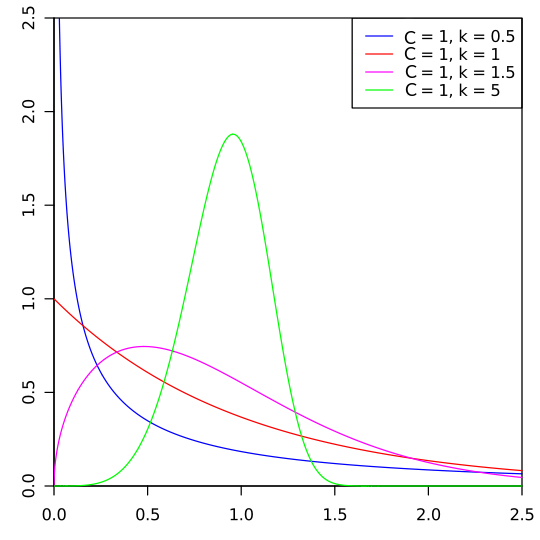
\includegraphics[height=50mm]{figures/weibull_distribution.png} 
    \caption{Función de distribución de probabilidad de Weibull}
    \vspace{-.25cm} 
    \caption*{Adaptación propia desde \cite{wikiWeibull}.}
    \label{fig:weibull_fig}
\end{figure}
 \subsection{Métodos numéricos}
 Tradicionalmente, se utilizan métodos numéricos para estimar los parámetros de la distribución de Weibull. En el artículo de Chang \cite{Chang10}, se realiza una comparación de seis métodos numéricos comúnmente utilizados para la obtención de $k$ y $c$. A continuación, se describen brevemente estos métodos:
 \begin{enumerate}
     \item \textbf{The Moment}: Se basa en la iteración numérica de las siguientes dos ecuaciones:
        \begin{align}
            \bar{v} &= c\Gamma(1 + \frac{1}{k})\\
            \sigma &= c[\Gamma(1 + \frac{2}{k}) - \Gamma^2(1 + \frac{1}{k})]^{\frac{1}{2}}
        \end{align}    
        Donde $\bar{v}$ es el promedio y $\sigma$ la desviación estándar de los datos de velocidad del viento.
    \item \textbf{Empirical}: Considerado un caso especial del método del momento. Los parámetros son calculados de la siguiente forma: 
        \begin{align}
            k &= (\frac{\sigma}{\bar{v}})^{-1.086}\\
            c &= \frac{\bar{v}}{\Gamma(1 + \frac{1}{k})}
        \end{align}    
    \item \textbf{Graphical}: Se ajustan rectas a los datos de velocidad del viento usando mínimos cuadrados. Con una doble transformación logarítmica, la función de distribución acumulativa queda:
        \begin{align}
            \ln\{-\ln[1- F(v)]\} = k\ln(v) - k\ln(c)
        \end{align}    
         Realizando un gráfico para $ln(v)$ en vez de $ln(-ln(1-F(v)))$, la pendiente de la recta que se ajusta mejor a los pares de datos es el parámetro de la forma de la distribución de Weibull. El parámetro de escala se obtiene por la intersección con la coordenada $y$.  
    \item \textbf{Maximum likelihood}: En este métodos, son necesarias muchas iteraciones. Los parámetros de Weibull están dado por:
        \begin{align}
            k &= [\frac{\sum_{i=1}^n v_i^k \ln(v_i)}{\sum_{i=1}^n v_i^k} - \frac{\sum_{i=1}^n \ln(v_i)}{n}]^{(-1)}\\
            c &= (\frac{1}{n}\sum_{i=1}^n v_i^k)^{\frac{1}{k}}
        \end{align}    
         Donde $v_i$ es la velocidad del viento en el paso $i$ y $n$ es el número de puntos de datos distintos de cero. 
    \item \textbf{Modified maximum likelihood}: Este método es utilizado si es que se tiene disponible los datos de velocidad del viento en una distribución de frecuencias. Los parámetros de Weibull son calculados como:
        \begin{align}
            k &= [\frac{\sum_{i=1}^n v_i^k \ln(v_i)f(v_i)}{\sum_{i=1}^n v_i^kf(v_I)} - \frac{\sum_{i=1}^n\ln(v_i)f(v_i)}{f(v \geq 0)}]^{-1}\\
            c &= [\frac{1}{f(v \geq 0)}\sum_{i=1}^n v_i^{k}f(v_i)]^{1/k}
        \end{align}
         Donde $v_i$ es la velocidad del viento central al intervalo $i$, $n$ es el número de intervalos. $f(v_i)$ es la frecuencia de la velocidad del viento dentro del intervalo $i$ y $f(v \geq 0)$ la probabilidad de que la velocidad del viento sea mayor o igual a cero.
    \item \textbf{Energy pattern factor method}: El factor del patrón de energía es definido como:
        \begin{align}
            E_{pf} = \frac{\bar{v^3}}{\bar{v}^3}
        \end{align}   
         Donde $\bar{v^3}$ es el promedio de las velocidades del viento cúbicas. Los parámetros de Weibull pueden ser calculados como:
        \begin{align}
            k &= 1 + \frac{3.69}{E_{pf}^2}\\
            c &= \frac{\bar{v}}{\Gamma(1 + \frac{1}{k})}
        \end{align}    
 \end{enumerate}     
 Estos métodos fueron comparados a través de pruebas de desempeño, con una simulación de Monte Carlo para este caso, y el análisis de los datos del viento con criterios tales como el test Kolmogorov-Smirnov, \emph{parameter error}, \emph{root mean square error} y el error de energía del viento. De ello, bajo distintas condiciones ciertos métodos se comportan mejor que otros ajustando la distribución de Weibull a los datos de prueba. Sin embargo, como se verá a continuación, una propuesta realizada para mejorar el ajuste a través del uso de la meta-heurística \emph{Particle Swarm Optimization}, mejora la calidad de los resultados comparado con estos métodos numéricos presentados.  
 \subsection{Particle Swarm Optimization}
 En Carneiro et al. \cite{Carneiro15}, se realiza un caso de estudio de las características del viento en las zonas costeras de Parnaiba y Maracanaú, y en una zona interior, Petrolina, en Brasil. Allí se explica la necesidad de obtener un modelo para el comportamiento estocástico del viento, de manera de poder evaluar el potencial energético de aquellas regiones. Como se menciona anteriormente, el modelo utilizado es la distribución de Weibull. Para ello, es preciso ajustar el modelo a los datos recolectados. Por esto, en el estudio mencionado, se propone un PSO para encontrar los parámetros $k$ y $c$ de la distribución de Weibull y a su vez mejorar la calidad de la solución comparada con los métodos numéricos tradicionales. Así, para lograr el objetivo, la función de aptitud se define como:
\begin{align}\label{eq:PSO_FO}
    \epsilon(v_i) = \frac{1}{2}\sum_{i=0}^{n}(f_{real}(v_i) - f_{weibull}(v_i))^2
\end{align}
Donde $\epsilon$, es el error cuadrático a minimizar entre los valores del histograma de datos y la función de distribución de Weibull.\\
El PSO utilizado es el modelo clásico presentado en la sección anterior, considerando los parámetros $w, c1$ y $c2$, sin embargo, para abolir la convergencia prematura, se establece que estos parámetros varíen durante la ejecución del algoritmo dentro de un rango definido ($w \in \{0.4, 0.9\}, c1$ y $c2 \in \{0, 2.5\}$), en donde se privilegia la exploración en el inicio de las iteraciones, para posteriormente favorecer la explotación al final de la ejecución.\\
Finalmente, para evaluar los resultados de la propuesta, se compara con el PSO con cinco de los seis métodos numéricos mencionados anteriormente utilizados para la estimación de los parámetros de Weibull: \emph{Moment Method} (M), \emph{Energy Method} (E), \emph{Energy Pattern Factor Method} (EPF), \emph{Energy Equivalent Method} (EE) y \emph{Maximum Likelihood} (ML). Además, para evaluar la eficiencia de los métodos, se utilizan tres \emph{test} estadísticos: \emph{correlation} (r), \emph{relative bias} (RB) y \emph{root mean square error} (RMSE).\\
Los resultados que se exponen en el trabajo citado son alentadores, demostrando que el PSO obtiene los mejores resultados de ajuste a los datos. Un ejemplo de esto es expuesto en la figura \ref{fig:pso_fit}.
\begin{figure}[h!]
    \centering    
    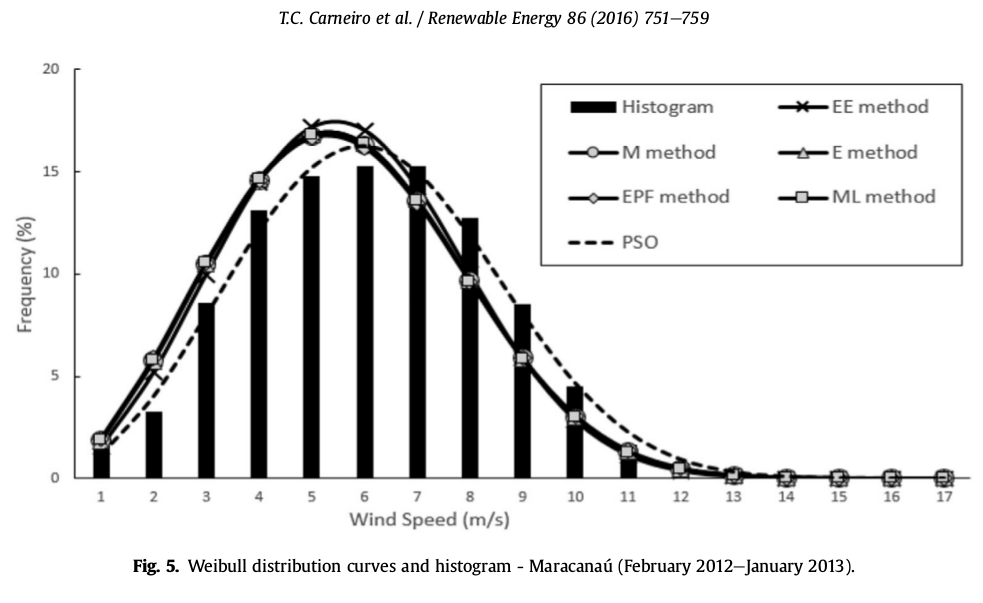
\includegraphics[height=50mm]{figures/pso_fit.png} 
    \caption{Distribución de Weibull con histograma - Maracanaú}
    \vspace{-.25cm} 
    \caption*{Creado por Carneiro et al.\cite{Carneiro15}.}
    \label{fig:pso_fit}
\end{figure}
En Kongnam et al. \cite{Kongnam15}, el PSO es utilizado para el problema del control de la velocidad de las turbinas de viento para maximizar la generación de energía. En este trabajo, se utiliza la distribución de Weibull para el modelado de la velocidad del viento. La construcción del PSO es llevada a cabo considerando el problema de la convergencia prematura, por lo que se desarrollan funciones que varían estos parámetros a lo largo de la ejecución.\\

\section{Dirección del viento}
La dirección del viento es información esencial para la investigación acerca de la energía eólica, dado que con esta, por ejemplo, se pueden ubicar de forma estratégica las turbinas que capturan la energía. En el resumen acerca de las energías renovables y sustentables\cite{Winddirelse15}, se explica que para identificar la dirección dominante del viento la función de densidad \emph{finite von Mises-Fisher} (FVMF) es utilizada para ajustarse a los datos. Para las pruebas, estos datos fueron obtenidos de cinco estaciones ubicadas en distintas zonas en la península de Malasia. La FVMF, de forma genérica, está definida de la siguiente forma:
\begin{align}
    f(x;\mu_{h}, k_{h}) = \sum_{h=1}^{H}(w_{h})\frac{k^{\frac{d}{2} - 1}}{(2\pi)^{\frac{d}{2}}I_{\frac{d}{2} - 1} (k)}e^{(k_h\mu_{h}^{T}x)}
\end{align}    
Donde $x=[cos(\theta_i), sin(\theta_i)]$, $\frac{k^{\frac{d}{2} - 1}}{(2\pi)^{\frac{d}{2}}I_{\frac{d}{2} - 1} (k)}$ es una constante de normalización, $d$ es la dimensión del vector aleatorio $x$ ($d = 2$, para este caso), $\mu_{h}$ y $k_h$ son el promedio direccional, parámetro de concentración para cada $h = 1, 2,...,H$ componente del FVFM y $w_h$ es el parámetro de mezcla (\emph{mixture parameter}).\\
Además, el parámetro de mezcla del FVMF está sujeto a la siguiente restricción:
\begin{align}
    0 \leq w_h \leq 1 \text{ y } \sum_{h=1}^{H} w_{h} = 1 \text{ para } (h=1,2,...,H) 
\end{align}
Para estimar los parámetros del FVMF, se sugiere utilizar el método \emph{expectation maximization}, debido a que los métodos regulares son incapaces de manejar la complejidad del modelo, consideraciones que se mencionan en el trabajo de Banerjee et al.\cite{Banerjee05}.\\
Por último, los resultados de este trabajo muestran que FVMF provee un razonable ajuste a diferentes conjunto de datos, obteniendo un modelo que explica más del $90\%$ de la variación de los datos, en este caso, obtenidos de estaciones ubicadas en la península de Malasia. En la figura \ref{fig:wind_dir_vonMises} se aprecia el ajuste del modelo a los datos, tanto la comparación con el histograma, como en su versión circular.\\
\begin{figure}[h!]
    \centering    
    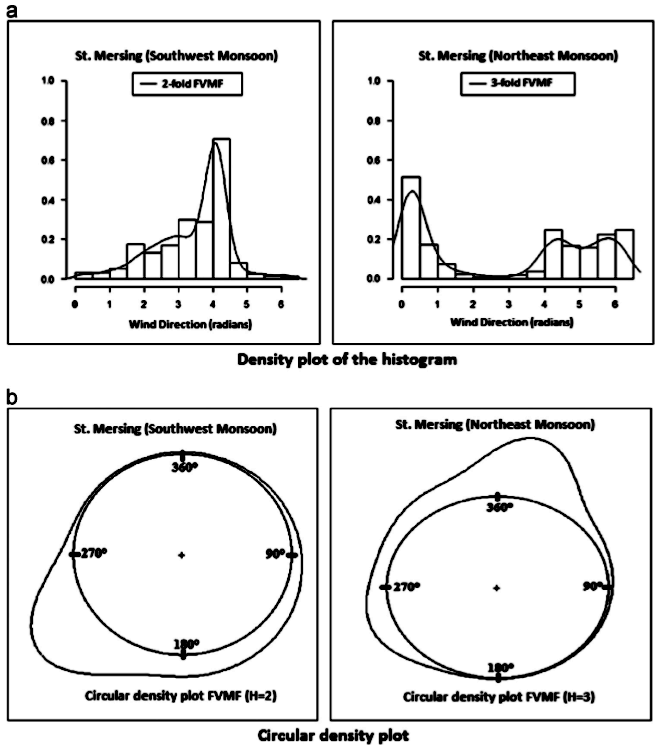
\includegraphics[height=100mm]{figures/wind_dir_vonMises.png} 
    \caption{Modelo de ajuste FVMV para suroeste y noreste en la estación Mersing}
    \vspace{-.25cm} 
    \caption*{Creado por \cite{Winddirelse15}.}
    \label{fig:wind_dir_vonMises}
\end{figure}

En el trabajo de Heckenbergerova et al.\cite{Heckenbergerova15}, se utiliza una estrategia diferente a la anteriormente mencionada. Basados en la ya mencionada meta-heurística inspirada en la biología, \emph{Particle Swarm Optimization}, proponen una forma distinta para encontrar un modelo de ajuste, utilizando la distribución estadística \emph{finite mixture of circular normal von Mises} (MvM), similar a la mencionada previamente.\\ 
En este caso, se define la distribución simple de \emph{von Mises} (SvM) como:
\begin{align}
    f(\theta; \mu, k) = \frac{1}{2{\pi}I_{0}(k)}e^{k cos(\theta - \mu)}
\end{align}    
Donde $k \geq 0$, $0 \leq \mu \leq 2\pi$, $0 \leq \theta \leq 2\pi$ y $I_0(k)$ representa la versión modificada de la función de Bessel de primera clase y orden cero:
\begin{align}
    I_0(k) = \frac{1}{\sqrt{2\pi}}\int_0^{2\pi} e^{k cos(\theta)} d\theta = \sum_{k=0}^{\infty} \frac{1}{(k!)^2}(\frac{k}{2})^{2k}
\end{align}    
Para $k=0$, la distribución SvM se vuelve uniforme alrededor de un círculo con todas las direcciones equi-probables. Cuando una colección de datos tiene más de una dirección predominante, es necesario utilizar una mezcla (\emph{mixture}) de distribuciones.
Así, la función de densidad de probabilidad \emph{finite mixture of simple von Mises} (MvM-pdf) queda como:
\begin{align}
    \phi(\theta; v) = \sum_{j=1}^{k} w_j \cdot f_j(\theta; \mu_j, k_j)
\end{align}    
Donde $k$ es el número de funciones de la mezcla, $j$ es el índice de una particular SvM-pdf con parámetros $\mu_j$ y $k_j$, $\theta$ es una variable angular ($0 \leq \theta \leq 2\pi$), y $v$ es un vector parámetro de la forma:
 \begin{align}\label{eq:sol_pso}
    v = (\mu, k, w) = (\mu_1, ..., \mu_k,k_1,...,k_k,w_1,...,w_k)
\end{align}
Para lograr el objetivo, se obtiene en primer lugar una aproximación numérica de los parámetros del MvM a partir de los datos recolectados de la dirección del viento, estrategia nombrada como estimación analítica en el trabajo de Heckenbergerova et al., para luego optimizarlos mediante el uso de un PSO, en su versión modificada, para evitar la convergencia prematura, en donde la solución está representada por una codificación del vector $\vec{v}$ mencionado anteriormente\ref{eq:sol_pso}.\\ 
Como test estadístico, es utilizado el \emph{Pearson's chi-squared goodness-off-fit}. Los resultados muestran la mejora que se logra a la estimación inicial, comparándose además con algoritmos genéticos. Sin embargo, estos no consiguen pasar el test estadístico impuesto, por lo que existe trabajo futuro  a realizar para mejorar la propuesta y lograr la precisión deseada.\\
Los resultados obtenidos para los datos recolectados en el aeropuerto de St John localizado en Newfoundland, Canadá, son apreciables en la figura \ref{fig:dir_pso}.
\begin{figure}[h!]
    \centering    
    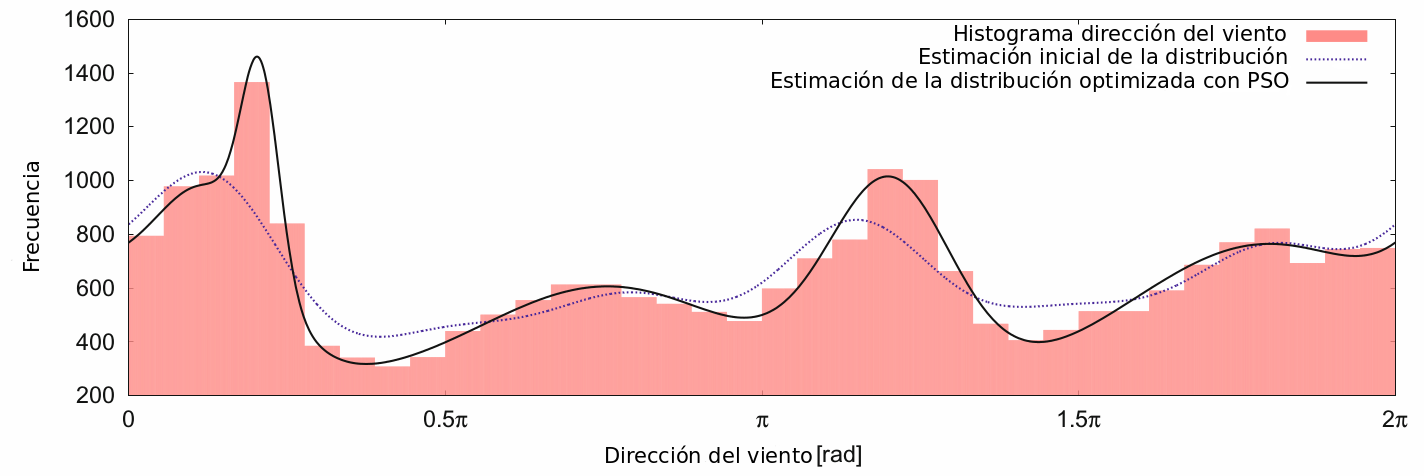
\includegraphics[height=50mm]{figures/dir_pso.png} 
    \caption{Ajuste dirección del viento, aeropuerto St. John}
    \vspace{-.25cm} 
    \caption*{Creado por Heckenbergerova et al.\cite{Heckenbergerova15}.}
    \label{fig:dir_pso}
\end{figure}


%!TEX root = main.tex

\chapter{Desarrollo de la solución}

\section{Velocidad del viento}
\subsection{Modelo Matemático} \label{ss:Modelo_Mat}
Como se adelanta anteriormente, para encontrar los parámetros de la distribución de Weibull que se ajusten a los datos de prueba se utilizará el \emph{Particle Swarm Optimization}. La función de distribución de Weibull está definida en la ecuación \ref{eq:weibull}. El PSO a utilizar está representado por la ecuación \ref{eq:PSO}. La función objetivo se describe con la fórmula \ref{eq:PSO_FO} y es aquella con la que se busca minimizar el error cuadrático entre la frecuencia real de los datos y la estimada por la distribución de Weibull. Los parámetros a encontrar $k$ y $c$ deben ser $\geq 0$ . Por último, a modo de favorecer la exploración al comienzo y la explotación al final de las iteraciones del PSO, se utilizará la recomendación de \cite{Carneiro15} para la variación de parámetros del enjambre:
\begin{align}\label{eq:VariationParameters}
    w(j) &= (1 - \frac{j}{iter_{max}})^{\alpha}(w_{max} - w_{min} + w_{min})\\
    c_{1}(j) &= (1 - \frac{j}{iter_{max}})^{\beta}(c_{1max} - c_{1min}) + c_{1min}\\
    c_{2}(j) &= (1 - \frac{j}{iter_{max}})^{\gamma}(c_{2min} - c_{2max}) + c_{2max}
\end{align}    
Donde $w_{max} = 0.9$ y $w_{min} = 0.4$, $c_{1max}$, $c_{2max}$ y $c_{1min}$, $c_{2min}$ son 2.5 y 0 respectivamente. Los parámetros $\alpha, \beta, \gamma$ son definidos como 0.5, 1.5 y 1.0 respectivamente. $iter_{max}$ es el máximo número de iteraciones.

\subsection{Representación}
Cada vector posición de las partículas del enjambre representa una solución candidata la cual varía dentro de cierto espacio de búsqueda definido por los límites de las componentes. Así, para el caso de los parámetros de la distribución de Weibull, la posición de las partículas está representada por los parámetros $k$ y $c$ quedando de la forma:
\begin{align}
    x = (k, c)
\end{align}    
Para ambos parámetros, se establecen los límites entre $0 \leq (k,c) \leq 20$, criterio que se basa en el trabajo de Carneiro et al. \cite{Carneiro15}. De esta forma, las partículas se moverán dentro de ese rango, manteniéndose en los lugares que minimizan la función objetivo, la cual representa el error de la predicción de Weibull versus los datos reales.\\
Así, para cada partícula se define una estructura que posee las siguientes propiedades: 
\begin{enumerate}\label{rep:Particle}
    \item Posición: vector de números flotantes de largo dos, los cuales representan la ubicación de la partícula dentro del espacio de búsqueda y sus componentes a los parámetros $k$ y $c$.
    \item Velocidad: vector de números flotantes que representan el cambio de valor de cada componente de la posición de la partícula en determinada iteración. Se actualiza en base a la ecuación de velocidad del PSO.
    \item Mejor resultado personal: vector flotante que guarda la mejor posición conseguida por la partícula durante las iteraciones transcurridas.    
\end{enumerate}        
Mientras que el enjambre, siendo esencialmente una estructura que posee referencia a todas las partículas, queda representado de la siguiente forma:
\begin{enumerate}\label{rep:Swarm}
    \item Partículas: Arreglo de referencias a las estructuras de partículas creadas.
    \item Mejor posición global: De todos los mejores resultados particulares a cada partícula, se almacena la mejor posición de todas. La que persiste al final del ciclo de iteraciones, es la solución final.
    \item W, C1 y C2: Son los parámetros de inercia, cognitivo y social respectivamente.    
\end{enumerate} 

\subsection{Descripción del algoritmo}
La lógica del algoritmo \ref{alg:pso} se basa en mover las partículas dentro del rango definido para los componentes de la solución hasta que todas las partículas se concentren en alguna zona que represente una buena solución al problema, no necesariamente el óptimo. Lo importante en cada iteración es actualizar o mover el enjambre, revisar y guardar las mejores soluciones y actualizar los parámetros de inercia, cognitivo y social que definen las velocidades.
%!TEX root = main.tex

\begin{algorithm}[h!]
\caption{PSO para el ajuste de los parámetros de la distribución de Weibull}
\label{alg:pso}
\begin{algorithmic}
\REQUIRE Datos de frecuencias de velocidades del viento.
\ENSURE Valores para los parámetros $k$ y $c$.
\STATE enjambre = inicializar(w,c1,c2)
\FOR{$i = 1$ to $Iter_{max}$}
\FOR{Each partículas en enjambre}
    \STATE actualizarVelocidadPartícula(partícula)
    \STATE actualizarPosiciónPartícula(partítucla)
    \STATE guardarMejorResultadoPartícula(partícula)
\ENDFOR
\STATE guardarMejorResultadoGlobal(enjambre)
\STATE actualizarParámetros(enjambre)
\ENDFOR
\STATE retornarMejorResultadoGlobal(enjambre).
\end{algorithmic}
\end{algorithm}

Las iteraciones fueron probadas hasta un máximo de 1000 y 50 partículas, (A excepción del experimento donde se consideraron todos los promedios diarios, 2013, 2014 y 2015, en el cual, se utilizaron 200 partículas). Los parámetros de $w$, $c1$ y $c2$ fueron definidos tal y como explica en el modelo matemático, en la sección \ref{ss:Modelo_Mat}.\\

\subsection{Experimentos}
Los experimentos fueron realizados con datos del viento obtenidos por la Armada de Chile para la región de Valparaíso en los años 2013, 2014 y 2015. Estos fueron tratados mediante \emph{scripts} desarrollados en python para obtener las frecuencias de las distintas velocidades del viento registradas a lo largo del año. Los datos se organizaban de la siguiente forma: Por cada año, se tiene una tabla en un archivo exel de cada mes, en donde se registra por cada fila los resultados de la medición de cada día. Las mediciones son registradas en un intervalo de tres horas, es decir, se tienen registros diarios para las 3:00, 6:00, 9:00, 12:00, 15:00, 18:00, 21:00 y 00:00 horas.\\
Un ejemplo es la tabla mostrada en la figura \ref{fig:example_data}.
 \begin{figure}[h!]
    \centering
    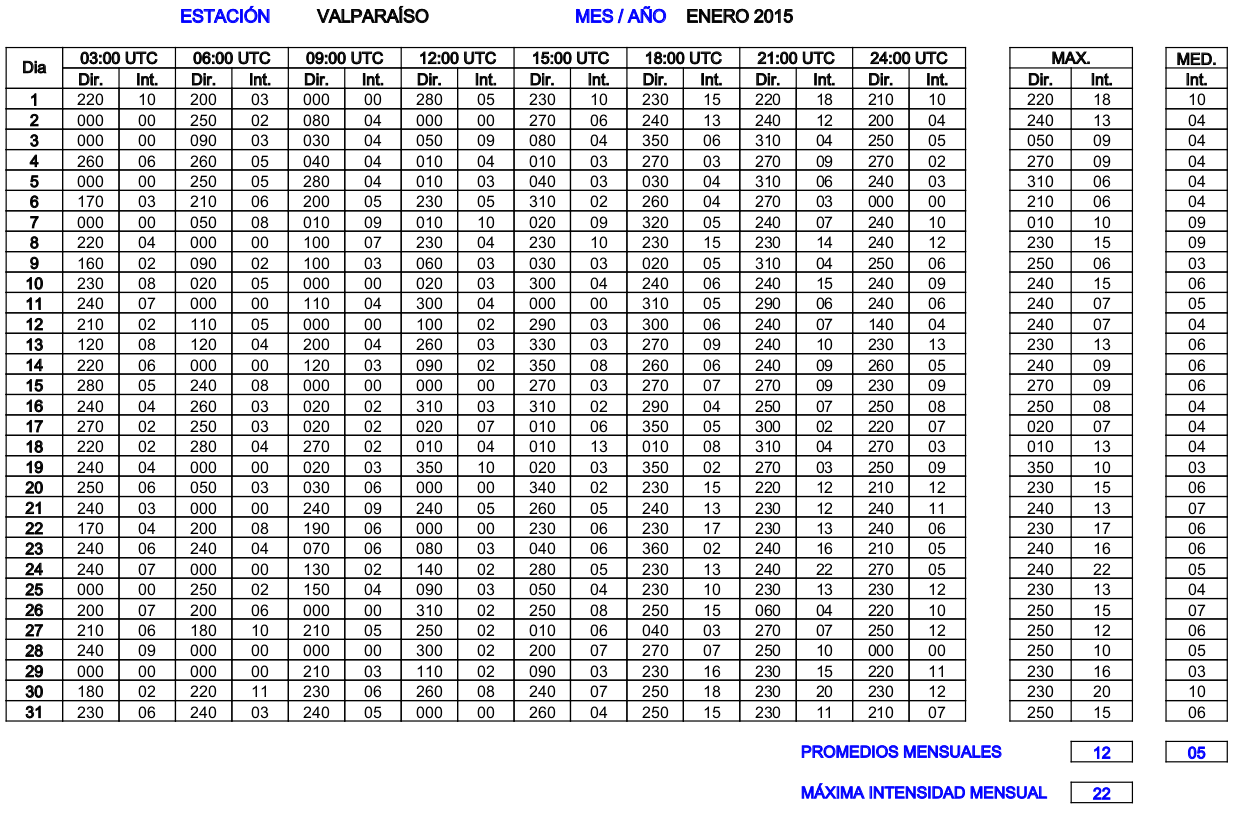
\includegraphics[height=100mm]{figures/example_data.png}
    \caption{Ejemplo colección de datos Enero Valparaíso 2015}
    \vspace{-.25cm}
    \caption*{Obtenido desde el Instituto Meteorológico de la Armada de Chile.}
    \label{fig:example_data}
 \end{figure}
El ajuste de la distribución de Weibull a estos datos de velocidad del viento se hizo considerando las siguientes configuraciones para el cálculo del
histograma de frecuencias:
\begin{enumerate}
	\item \textbf{Todos los años}. Se considera el promedio diario de velocidad del viento como dato unitario para el cálculo de las frecuencias, considerando
	todos los días en el intervalo de Enero del 2013 hasta Diciembre del 2015.
	\item \textbf{Anual}. Se considera el promedio diario de velocidad del viento como dato unitario para el cálculo de las frecuencias en
	un lapso anual (2013, 2014 y 2015).
	\item \textbf{Por temporada}. Se considera el promedio diario de velocidad del viento como dato unitario para el cálculo de las frecuencias en
	un lapso de tres meses (Enero - Marzo ; Abril - Junio; Julio - Septiembre; Octubre - Diciembre).
	\item \textbf{Datos brutos}. Se considera cada medición realizada (8 por día) como dato unitario, en un lapso de un año.
\end{enumerate}

Una vez obtenido los datos de frecuencias, se procede a aplicar el algoritmo PSO obteniendo los parámetros de ajuste $k$ y $c$. De esta manera, se evalúa la calidad del modelo generado (distribución de Weibull), para las distintas configuraciones mediante gráficos y los siguientes test estadísticos (utilizados en el trabajo de Carneiro et al. \cite{Carneiro15}):
\begin{enumerate}
    \item \emph{Root Mean Square Error}
        \begin{align}
            RMSE = \sqrt{\frac{\sum_{i=1}^{N}(X_i - Y_i)^2}{N}}
        \end{align}    
    \item \emph{Correlation}
        \begin{align}
            r = \frac{\sum_{i=1}^{N}(X_i - X_{med})\cdot(Y_i - Y_{med})}{\sqrt{\sum_{i=1}^{N}(X_i - X_{med})^2}\cdot\sqrt{\sum_{i=1}^{N}(Y_i - Y_{med})^2}}
        \end{align}    
    \item \emph{Relative Bias}
        \begin{align}
            RB = \frac{X_{med} - Y_{med}}{Y_{med}}  
        \end{align}    
\end{enumerate}        
Donde $N$ es el número de datos, $Y_i$ la frecuencia de dichos datos, $X_i$ la frecuencia entregada por la distribución de Weibull, $X_{med}$ la media de $X_i$ e $Y_{med}$ la media de $Y_i$. \\

Las pruebas fueron realizadas en un computador con sistema operativo Ubuntu 16.04 64-bit, 3.8 GB de memoria y procesador doble núcleo Intel Pentium 2.60 GHz. 

\section{Dirección del viento}
\subsection{Modelo Matemático} 
Como se comenta anteriormente, la distribución de densidad de probabilidad que se utilizará para describir la distribución de datos de dirección del viento
es la \emph{mixture von mises distribution} descrita en \ref{eq:mixtureVonMises}, la cual consiste básicamente en una combinación lineal de la \emph{simple von Mises distribution} descrita en \ref{eq:simpleVonMises}.\\ 
De forma preliminar, los datos se ordenan en un histograma de densidad con el cual se obtiene un esqueleto de la distribución de densidad de probabilidad. Posteriormente se requieren encontrar los parámetros de ajuste $\mu_j$, $k_j$ y $w_j$ para cada $j$-ésima \emph{simple von Mises distribution}. La forma en que
se realiza esto último en este trabajo está basado en Heckenbergerova et al. \cite{Heckenbergerova15} y se describe a continuación.\\
Para la construcción del histograma se divide el rango de datos que va de 0 a $2\pi$ en $T$ clases con frecuencia $O_i$ la cual representa la suma de las observaciones en el rango de la clase $T$. Posteriormente se definen $k$ sectores del mismo largo desde las $T$ clases, relacionados al número de direcciones de viento predominantes (o con mayor frecuencia). Esto define el número de funciones de von Mises a utilizar. La estimación de $k$ se realiza mediante la observación del histograma generado, un análisis cualitativo de las direcciones predominantes en los datos.\\
Para la aproximación inicial de los parámetros de la \emph{mixture von mises distribution} se utiliza una estimación numérica basada en los datos recolectados acerca de la dirección del viento.\\
Sea $j \in \{1 ... k\}$ el subíndice del sector representado por la $j$-ésima función de von Mises.\\
La dirección del viento predominante $\mu_j$ se estima de la siguiente forma:
\begin{align}\label{eq:Prevailing_Param}
    \mu_j &= 
        \left\{
            \begin{array}{ll}
                arctan(\frac{s_j}{c_j})  & s_j \geq 0, c_j > 0\\
                \frac{\pi}{2} & s_j > 0, c_j = 0\\
                \pi + arctan(\frac{s_j}{c_j}) & c_j < 0\\
                \pi & s_j > 0, c_j = -1\\
                2\pi + arctan(\frac{s_j}{c_j}) & s_j < 0, c_j > 0\\
                3\frac{\pi}{2} & s_j < 0, c_j = 0\\
            \end{array}
        \right.
\end{align}
En donde $s_j$ y $c_j$ representan el seno y coseno promedio del sector $j$.\\
Tradicionalmente, se estima el parámetro de concentración $k_j$ con la ecuación:
\begin{align}\label{eq:Implicit_Param}
    \frac{I_1(k_j)}{I_0(k_j)} = \sqrt{s_j^2 + c_j^2}
\end{align}
Donde $I_1(k_j)$ es la función modificada de Bessel de primera clase y orden 1.
Para evitar la resolución de la ecuación implícita \ref{eq:ImplicitK} se utiliza la propuesta realizada en el trabajo previamente citado de Heckenbergerova et al. con lo cual el parámetro $k_j$ puede ser aproximado por:\\
\begin{align}
    |k_j| = \{23.29041409 - 16.8617370\sqrt[4]{s_j^2 + c_j^2}\} 
\end{align}
Los pesos iniciales $w_j$ son aproximados como: \\
\begin{align}\label{eq:Weight_Param}
    w_j = \frac{\sum_{i=J_l}^{J_u} O_i}{\sum_{i=1}^{T} O_i}
\end{align}

Donde $J_l$ y $J_u$ son los índices de los bordes del sector $j$.\\
Esta estimación inicial de los parámetros de la \emph{mixture von mises distribution} es mejorada mediante la meta-heurística \emph{Particle Swarm Optimization}. Para el PSO se utiliza la representación descrita en \ref{eq:PSO} y la modificación a este sugerida en Carneiro et al. \cite{Carneiro15} descrita previamente en \ref{eq:VariationParameters}.\\
La función objetivo para el PSO es el test estadístico $\chi^2$ descrito en \cite{Heckenbergerova15} como sigue a continuación:
\begin{align}\label{eq:FO_Direction}
    \chi^2 = \sum_{i=1}^{T}\frac{(O_i - np_{i})^2}{np_i}
\end{align}
Donde $T$ es el número de clases de frecuencia definido para construir el histograma, $n$ es la suma de las frecuencias observadas $O_i$ y $p_i$ es la probabilidad teórica de cada clase de frecuencia predicha por el modelo ajustado.\\
Para el cálculo del $p_i$ se utiliza:
\begin{align}
    p_i = \int_{l_i}^{u_i} f(x) dx
\end{align}
Donde $u_i$ y $l_i$ son los bordes de la $i$-ésima clase de frecuencia.\\
La forma de la solución a encontrar es descrita en \ref{eq:sol_pso}. Esta es restringida por la condición para los pesos de la \emph{mixture von mises distribution}, la cual obliga a que se deba cumplir que la suma de los pesos sea igual a 1, como se describe en \ref{eq:WeightConstraint}.
\subsection{Representación}\label{sec:Representacion}
La representación del PSO es similar al utilizado para el ajuste de la distribución de datos de velocidad del viento. Las partículas y el enjambre están representados por \ref{rep:Particle} y \ref{rep:Swarm} respectivamente.\\
La solución para el PSO que mejora la estimación inicial de los parámetros para la \emph{mixture von Mises distribution} está representado por un vector $v$ en el cual se encuentran los valores para todos los parámetros de cada \emph{simple von Mises distribution}. Estos valores están codificados para que el algoritmo se mueve en el rango desde 0 a 1.\\
El vector solución tiene la forma:
\begin{align}
    v = (\overbrace{v_1,...,v_k}^{\mu},\overbrace{v_{k+1},...,v_{2k}}^{k},\overbrace{v_{2k+1},...,v_{n}}^{w}).
\end{align}
El parámetro $\mu$ está representado en el rango $i \in \{1,...,k\}$ y para ser decodificado debe ser escalado por $2\pi$.\\
El parámetro $k$ está representado en el rango $i \in \{k+1,...,2k\}$ y para ser decodificado debe ser escalado por $[0, 700]]$.\\
El parámetro $w_j$ está representado en el rango $i \in \{2k+1,...,n\}$ cuyos valores van en el rango $[0,1]$.

\subsection{Descripción del algoritmo}
El algoritmo para el ajuste de la función de densidad de probabilidad para la dirección del viento se basa en la propuesta de Heckenbergerova et al. \cite{Heckenbergerova15}.\\ 
Como se ha ido vislumbrado, consiste en dos fases. La primera, una aproximación basada en la estimación numérica de los parámetros requeridos para la \emph{mixture of von Mises distribution} a través de operaciones simples con los datos recolectados, y la segunda, una mejora de la solución inicial obtenida en la fase anterior mediante el uso de la meta-heurística \emph{Particle Swarm Optimization}. \\
A continuación se describe el algoritmo para la aproximación inicial de la solución.
%!TEX root = main.tex

\caption{Aproximación inicial de los parámetros de la \emph{mixture von Mises distribution}}
\begin{algorithmic}
\REQUIRE Datos de frecuencias de la dirección del viento.
\REQUIRE K, Cantidad de \emph{simple von Mises distribution}.
\REQUIRE T, clases de frecuencias.
\REQUIRE D, Total de datos.
\ENSURE Valores para los parámetros $\mu_j$, $k_j$ y $w_j$, para cada $j \in \{1,...,k\}$.
\STATE sol = inicializarVectorSolución(3*K)
\FOR{$j = 0$ to $K$}

\STATE datos$_j$ = datosEnRango($j*D/K$)
\STATE s$_j$ = obtenerSenoPromedio(datos$_j$)
\STATE c$_j$ = obtenerCosenoPromedio(datos$_j$)
\STATE u$_j$ = obtenerDirecciónPredominante(s$_j$,c$_j$)
\STATE k$_j$ = obtenerConcentración(s$_j$, c$_j$)
\STATE w$_j$ = obtenerPeso($j*(T/K)$, $(j + 1)*(T/K)$)
\STATE addToSolution(sol, u$_j$, k$_j$, w$_j$)

\ENDFOR
\STATE retornarSoluciónInicial(sol).
\end{algorithmic}
En donde la estimación de los parámetros se realiza como se describe en \ref{eq:Prevailing_Param} para los $\mu_j$, \ref{eq:Implicit_Param} para los $k_j$ y \ref{eq:Weight_Param} para los pesos $w_j$.
Una vez obtenida la aproximación inicial se procede a mejorar esta mediante el uso del PSO.
%!TEX root = main.tex
\caption{PSO para la mejora de la aproximación de los parámetros de la \emph{mixture von Mises distribution}}
\begin{algorithmic}
\REQUIRE Datos de la dirección del viento.
\REQUIRE Solución inicial para el ajuste de la \emph{mixture von Mises distribution}.
\ENSURE Solución inicial mejorada.
\STATE enjambre = inicializar(w,c1,c2)
\FOR{$i = 1$ to $Iter_{max}$}
\FOR{Each partículas en enjambre}
    \STATE actualizarVelocidadPartícula(partícula)
    \STATE actualizarPosiciónPartícula(partítcula)
    \STATE revisarLímitesPosición(partícula)
    \STATE guardarMejorResultadoPartícula(partícula)
\ENDFOR
\STATE guardarMejorResultadoGlobal(enjambre)
\STATE actualizarParámetros(enjambre)
\ENDFOR
\STATE retornarMejorResultadoGlobal(enjambre).
\end{algorithmic}
El algoritmo es bastante similar en estructura al desarrollado para la dirección del viento \ref{alg:pso}. Sin embargo,
existen diferencias importantes, relevantes al problema actual que se destacarán a continuación.\\
Para la inicialización de las partículas, se realizaron pequeñas perturbaciones a la solución inicial tal y como se sugiere en Heckenbergerova et al. \cite{Heckenbergerova15}. Esto evita que la solución escape a zonas que tengan un buen resultado en la función objetivo, pero que la forma escape a la del histograma. Debido a que la función objetivo definida \ref{eq:FO_Direction} mide las diferencias de frecuencias entre los datos reales y los teóricos, es decir, las áreas de las barras del histograma de densidad versus el área bajo la curva de la distribución de probabilidad en algún intervalo, más de una forma de la curva podría parecer una buena solución. (referencia imágen) Por ello, la idea es mantener la forma inicial encontrada, mejorándola sin deformarla. Así, las perturbaciones iniciales a los valores entre 0 y 1  de las posiciones de las partículas eran del orden de $~ 10^{-3}$.\\
La forma en que se cuidaron las condiciones de borde consistieron en limitar el avance de las partículas a los bordes 0 y 1 manteniéndolos en dichos valores si es que se excedían a ellos.\\
Para cuidar la restricción de pesos se normalizaran los valores determinados en cada iteración, es decir, se suman todos los valores $w_j$ y se ponderan dichos valores por el recíproco de la suma obtenida.\\
Debido a que la función objetivo implica determinar la frecuencia teórica, es necesario determinar la probabilidad
de cierto rango de direcciones mediante el cálculo del área bajo la curva de la distribución de densidad de probabilidad para luego ser multiplicada por la suma del total de datos y así obtener el valor requerido. Por ende, para el cálculo de la integral se utilizaron sumas de Riemann con una partición conveniente al desempeño del algoritmo y la precisión requerida.\\
Finalmente, la solución obtenida es decodificada tal y como se explica en la sección anterior \ref{sec:Representacion}.
\subsection{Experimentos}
* Test estadisticos y gráficoss

%!TEX root = main.tex

\chapter{Análisis y conclusiones}

\section{Resultados y conclusiones}
\subsection{Análisis de los resultados}
Los gráficos \ref{fig:data_valpo_13}, \ref{fig:data_valpo_14} y \ref{fig:data_valpo_15} muestran la distribución de dato de velocidad del viento en Valparaíso a lo largo de los meses del año y las horas del día, lo cual permite saber, por ejemplo, en que época del año el viento alcanza las velocidades más altas.\\
Las figuras \ref{fig:pso_valpo_13}, \ref{fig:pso_valpo_14} y \ref{fig:pso_valpo_15} muestran el ajuste de la distribución de Weibull a los histogramas de datos del viento, con los parámetros $k$ y $c$  que se muestran en la tabla \ref{table:stadistical_tests} determinados por el PSO. A simple vista, el ajuste parece de buena calidad, lo cual es corroborado por los datos estadísticos obtenidos con los test previamente mencionados (RMSE, r, RB), expuestos en la tabla \ref{table:stadistical_tests}. Si se compara con la precisión conseguida en el trabajo de Carneiro et al. \cite{Carneiro15}, se aprecia que el ajuste conseguido es levemente más impreciso, sobre todo en lo relativo al test RB. Esto podría deberse a la distribución de los datos de Valparaíso, los cuales, comparativamente hablando, son más concentrados en las velocidades  3 y 4 $[m/s]$.\\
Para confirmar el supuesto relativo a los datos, se calcularon los parámetros de Weibull utilizando el método numérico EM (Empirical Method) para los datos de Valparaíso 2015, cuyo ajuste se aprecia en la figura \ref{fig:em_valpo_15}. Tal y como se aprecia en los datos estadístico de la tabla \ref{table:stadistical_tests}, el ajuste conseguido es de menor calidad.\\
\begin{figure}[h!]
    \centering
    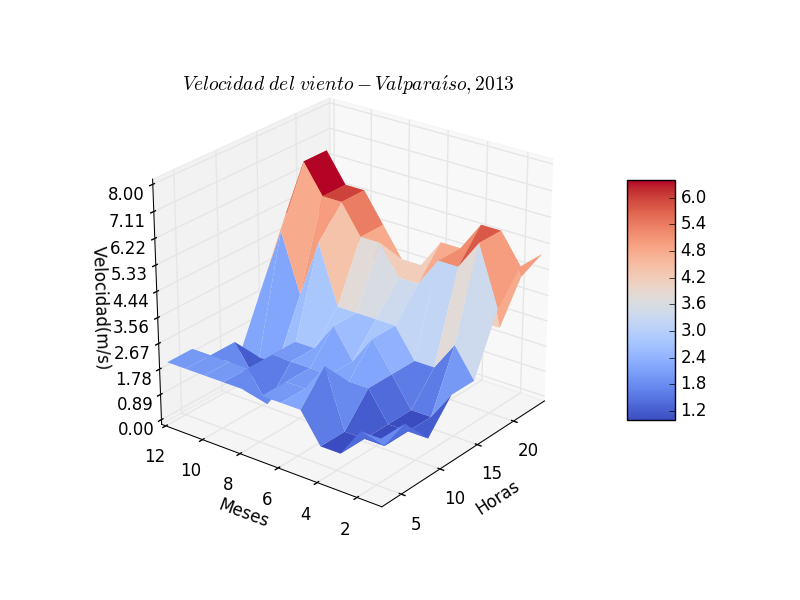
\includegraphics[height=75mm]{figures/3d_data_2013.png}
    \caption{Superficie datos Valparaíso 2013}
    \vspace{-.25cm}
    \caption*{Fuente: Elaboración Propia.}
    \label{fig:data_valpo_13}
\end{figure}
\begin{figure}[h!]
    \centering
    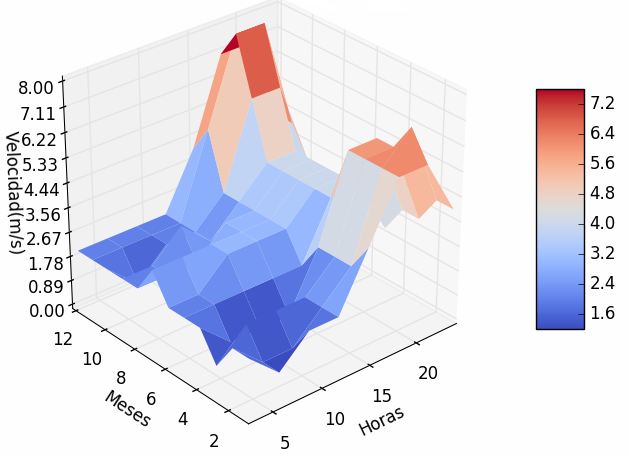
\includegraphics[height=75mm]{figures/3d_data_2014.png}
    \caption{Superficie datos Valparaíso 2014}
    \vspace{-.25cm}
    \caption*{Fuente: Elaboración Propia.}
    \label{fig:data_valpo_14}
\end{figure}
\begin{figure}[h!]
    \centering
    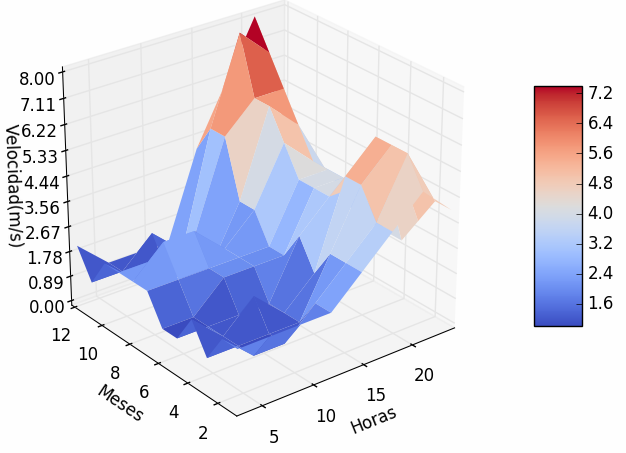
\includegraphics[height=75mm]{figures/3d_data_2015.png}
    \caption{Superficie datos Valparaíso 2015}
    \vspace{-.25cm}
    \caption*{Fuente: Elaboración Propia.}
    \label{fig:data_valpo_15}
\end{figure}
\begin{figure}[h!]
    \centering
    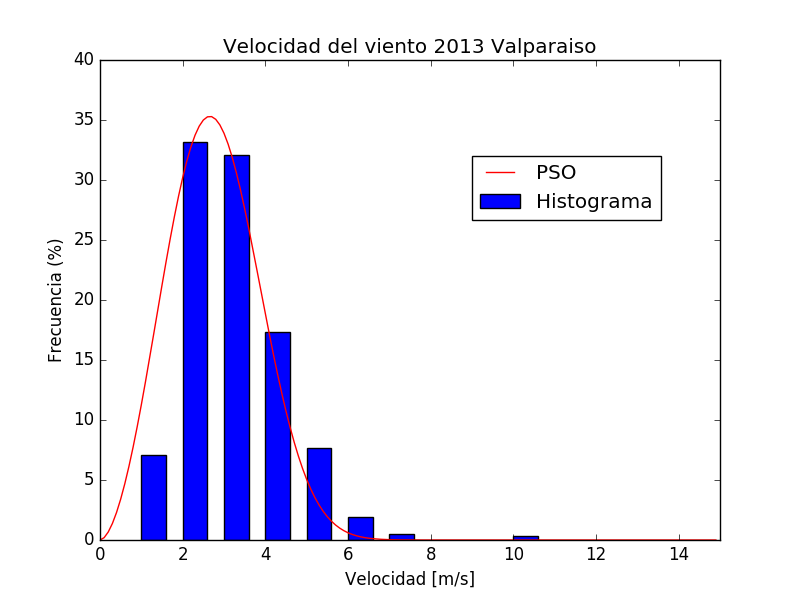
\includegraphics[height=75mm]{figures/result_2013.png}
    \caption{Ajuste con PSO a datos Valparaíso 2013}
    \vspace{-.25cm}
    \caption*{Fuente: Elaboración Propia.}
    \label{fig:pso_valpo_13}
\end{figure}
\begin{figure}[h!]
    \centering
    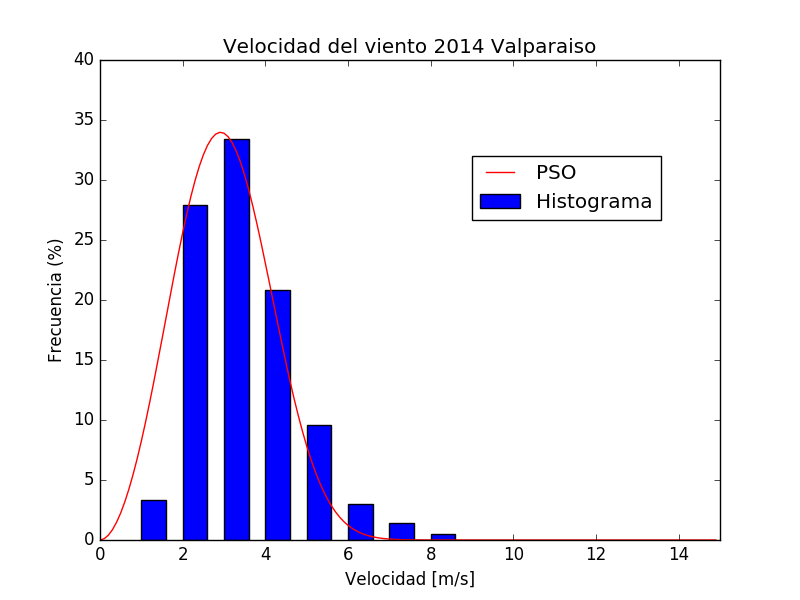
\includegraphics[height=75mm]{figures/result_2014.png}
    \caption{Ajuste con PSO a datos Valparaíso 2014}
    \vspace{-.25cm}
    \caption*{Fuente: Elaboración Propia.}
    \label{fig:pso_valpo_14}
\end{figure}
\begin{figure}[h!]
    \centering
    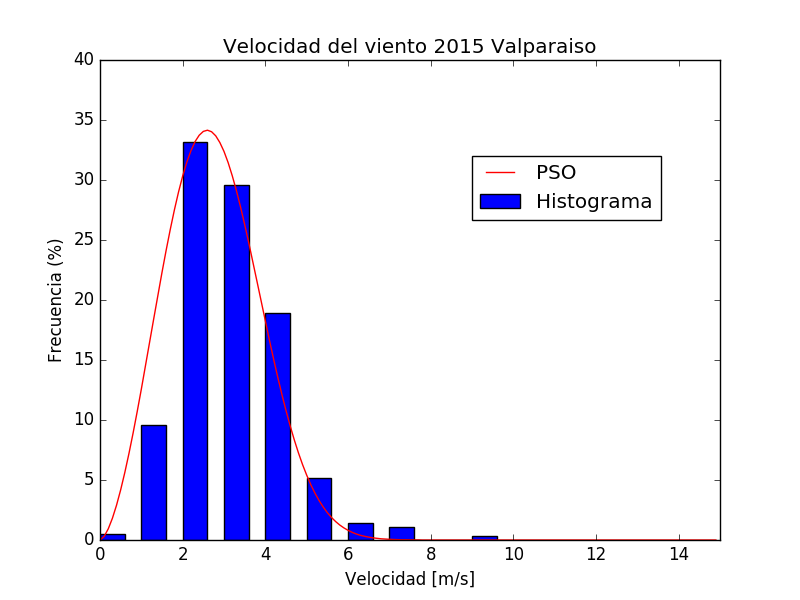
\includegraphics[height=75mm]{figures/result_2015.png}
    \caption{Ajuste con PSO a datos Valparaíso 2015}
    \vspace{-.25cm}
    \caption*{Fuente: Elaboración Propia.}
    \label{fig:pso_valpo_15}
\end{figure}

%Desde acá

\begin{figure}[h!]
    \centering
    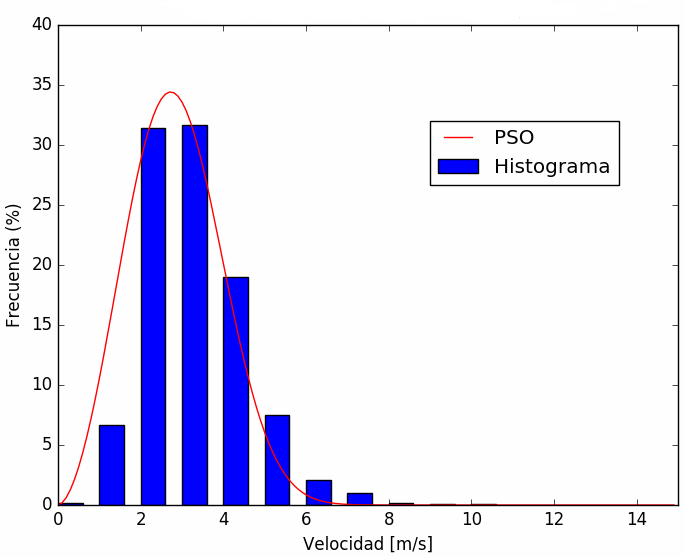
\includegraphics[height=75mm]{figures/result_13-14-15.png}
    \caption{Ajuste con PSO a datos Valparaíso 2015, 2014 y 2013}
    \vspace{-.25cm}
    \caption*{Fuente: Elaboración Propia.}
    \label{fig:pso_valpo_15_14_13}
\end{figure}
\begin{figure}[h!]
    \centering
    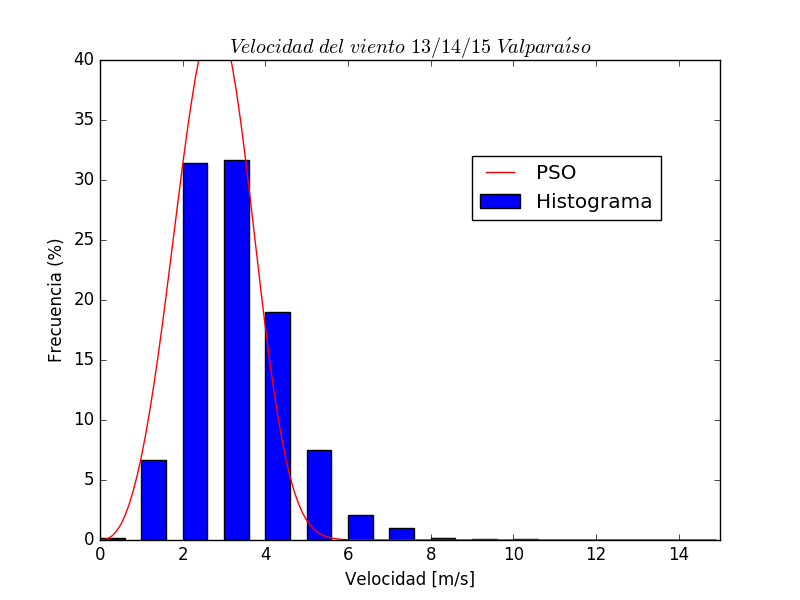
\includegraphics[height=75mm]{figures/result_13-14-15_low_quality.png}
    \caption{Ajuste con PSO a datos Valparaíso 2015, 2014 y 2013, baja calidad}
    \vspace{-.25cm}
    \caption*{Fuente: Elaboración Propia.}
    \label{fig:pso_valpo_15_14_13_lq}
\end{figure}
\begin{figure}[h!]
    \centering
    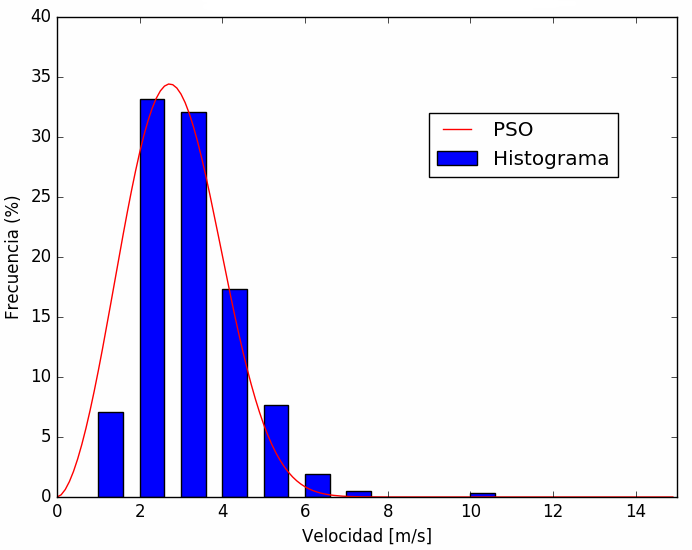
\includegraphics[height=75mm]{figures/result_2013_fit_all_data.png}
    \caption{Ajuste con PSO (Con todos los datos) a datos Valparaíso 2013}
    \vspace{-.25cm}
    \caption*{Fuente: Elaboración Propia.}
    \label{fig:pso_valpo_13_all_data}
\end{figure}
\begin{figure}[h!]
    \centering
    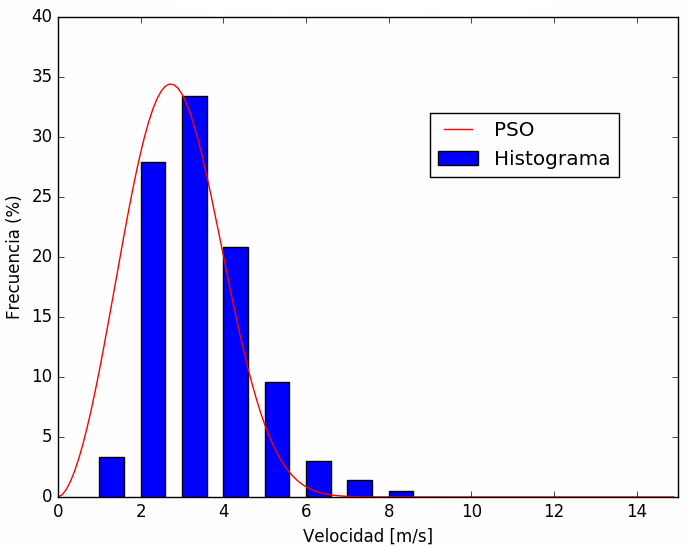
\includegraphics[height=75mm]{figures/result_2014_fit_all_data.png}
    \caption{Ajuste con PSO (Con todos los datos) a datos Valparaíso 2014}
    \vspace{-.25cm}
    \caption*{Fuente: Elaboración Propia.}
    \label{fig:pso_valpo_14_all_data}
\end{figure}
\begin{figure}[h!]
    \centering
    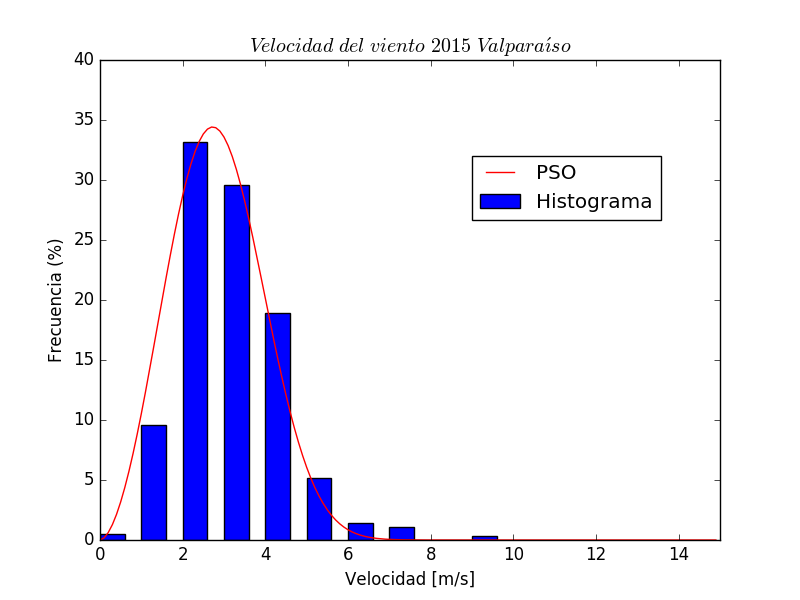
\includegraphics[height=75mm]{figures/result_2015_fit_all_data.png}
    \caption{Ajuste con PSO (Con todos los datos) a datos Valparaíso 2015}
    \vspace{-.25cm}
    \caption*{Fuente: Elaboración Propia.}
    \label{fig:pso_valpo_15_all_data}
\end{figure}
\begin{figure}[h!]
    \centering
    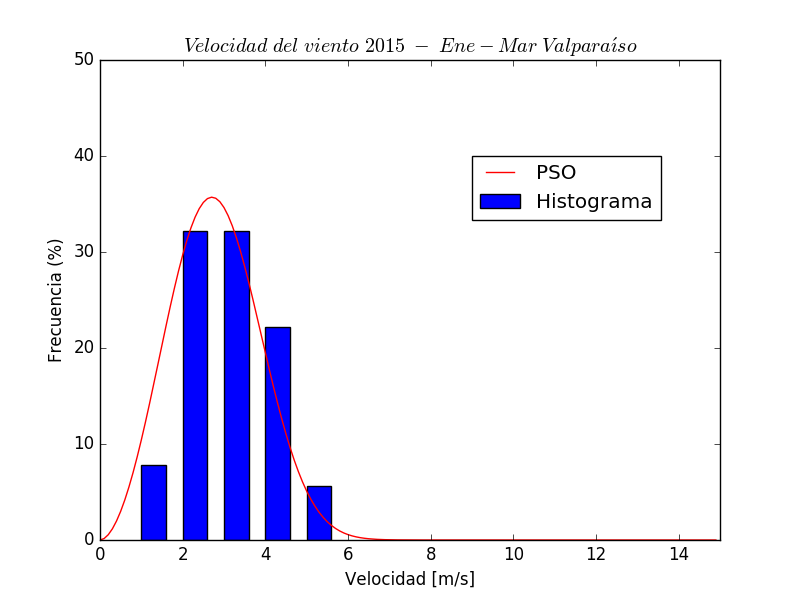
\includegraphics[height=75mm]{figures/result_2015_Ene-Mar.png}
    \caption{Ajuste con PSO a datos Valparaíso 2015, Enero - Marzo}
    \vspace{-.25cm}
    \caption*{Fuente: Elaboración Propia.}
    \label{fig:pso_valpo_15_ene_mar}
\end{figure}
\begin{figure}[h!]
    \centering
    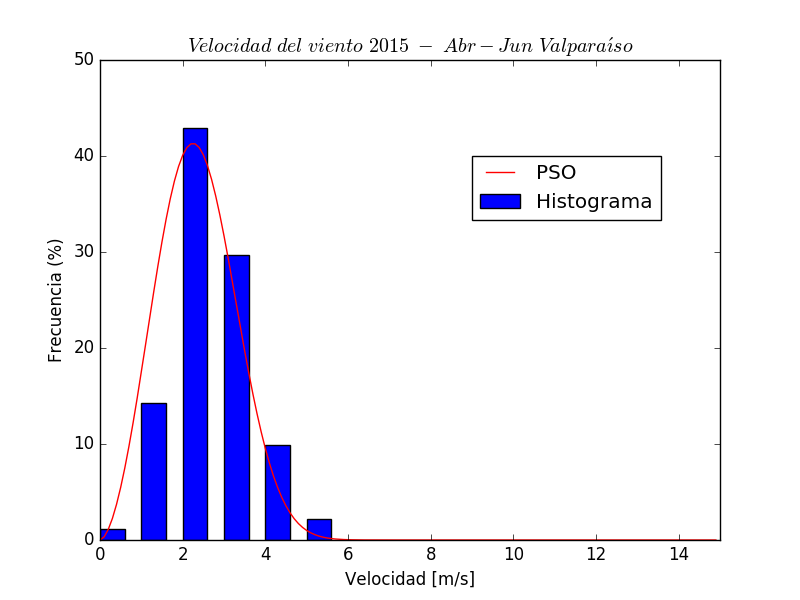
\includegraphics[height=75mm]{figures/result_2015_Abr-Jun.png}
    \caption{Ajuste con PSO a datos Valparaíso 2015, Abril - Junio}
    \vspace{-.25cm}
    \caption*{Fuente: Elaboración Propia.}
    \label{fig:pso_valpo_15_abr_jun}
\end{figure}
\begin{figure}[h!]
    \centering
    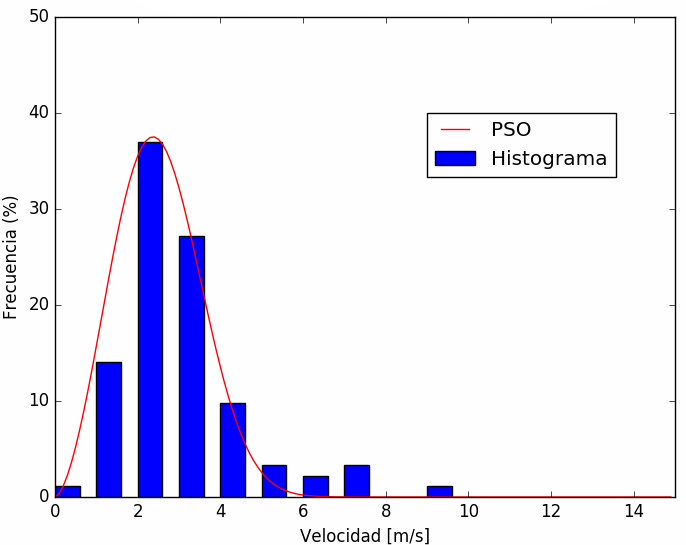
\includegraphics[height=75mm]{figures/result_2015_Jul-Sep.png}
    \caption{Ajuste con PSO a datos Valparaíso 2015, Julio - Septiembre}
    \vspace{-.25cm}
    \caption*{Fuente: Elaboración Propia.}
    \label{fig:pso_valpo_15_jul_sep}
\end{figure}
\begin{figure}[h!]
    \centering
    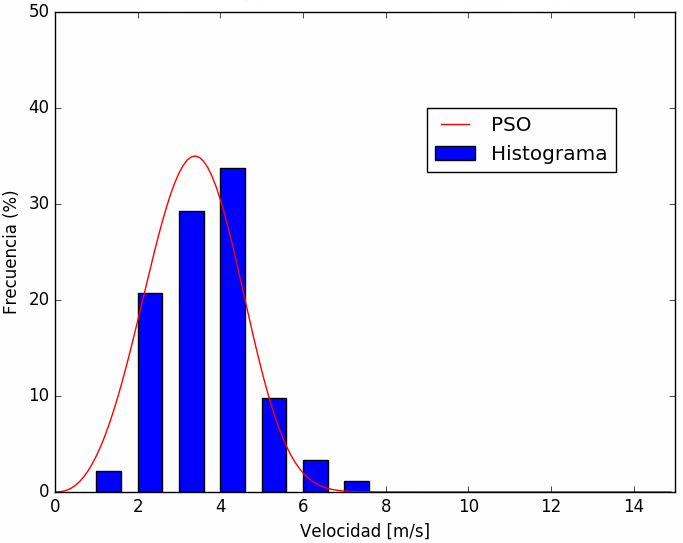
\includegraphics[height=75mm]{figures/result_2015_Oct-Dic.png}
    \caption{Ajuste con PSO a datos Valparaíso 2015, Octubre - Diciembre}
    \vspace{-.25cm}
    \caption*{Fuente: Elaboración Propia.}
    \label{fig:pso_valpo_15_oct_dic}
\end{figure}
\begin{figure}[h!]
    \centering
    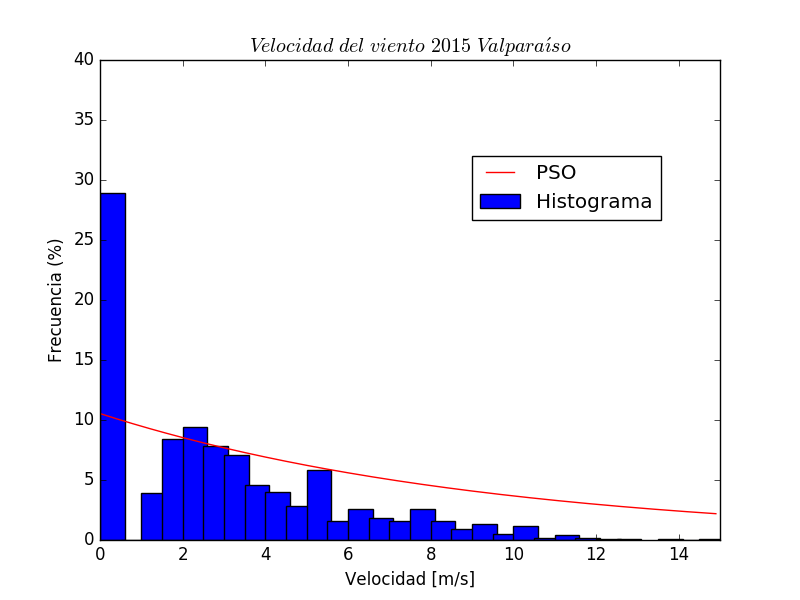
\includegraphics[height=75mm]{figures/result_2015_all_data.png}
    \caption{Ajuste con PSO a datos (cifras puras) Valparaíso 2015, 2014, 2013}
    \vspace{-.25cm}
    \caption*{Fuente: Elaboración Propia.}
    \label{fig:pso_valpo_15_oct_dic}
\end{figure}


\begin{table}[htb!]
    \centering
    \caption{Tabla de tests estadísticos}
    \label{table:stadistical_tests}
    %\resizebox{\columnwidth}{!}{
    \begin{tabular}{|c|c|c|c|c|c|c|}
        \hline
        \textbf{Método} & \textbf{Período} & \textbf{k} & \textbf{c} & \textbf{RMSE} & \textbf{r} & \textbf{RB}\\
        \hline
        PSO & 2013 & 2.78 & 3.12 &0.0226585230791 & 0.984353070415 & 0.00197971468299\\
        PSO & 2014 & 2.91 & 3.37 &0.0232779965263 & 0.982087745069 & 0.000754465101398\\
        PSO & 2015 & 2.65 & 3.10 &0.0164721412159 & 0.992323803649 & 0.00302918178445\\
        \hline
        PSO (Intento 1) & 2015-14-13 & 3.47 & 3.07 & 0.0360794587206 & 0.975240385258 & 0.000411212628513\\
        PSO (Intento 2) & 2015-14-13 & 2.78 & 3.20 & 0.016175531561 & 0.994989105807 & 0.00190916669626\\
        \hline
        PSO (Intento 2) & 2013 & 2.78 & 3.20 & 0.0240448436122 & 0.981963054492 & 0.00192186034284\\
        PSO (Intento 2) & 2014 & 2.78 & 3.20 & 0.0301463089474 & 0.970662237238 & 8.89024791609e-05\\
        PSO (Intento 2) & 2015 & 2.78 & 3.20 & 0.0202342934641 & 0.98662798667 & 0.00192175053173\\
        \hline
        PSO & Ene-Mar & 2.85 & 3.15 & 0.0230380400157 & 0.982158006469 & 0.00641888742608\\
        PSO & Abr-Jun & 2.76 & 2.65 & 0.0204300909755 & 0.993857185938 & 0.00303620481316\\
        PSO & Jul-Sep & 2.66 & 2.83 & 0.0251002816356 & 0.985858767021 & 0.00443453471038\\
        PSO & Oct-Dic & 3.40 & 3.75 & 0.0260278634297 & 0.978479679326 & 0.000716653529598\\
        \hline 
        PSO (datos brutos) & 2015 & 1.00 & 9.49 & 0.0451794472583 & 0.751732944794 & 0.676094670465\\ 
    \end{tabular}
    %}   
\end{table}
\pagebreak
\subsection{Conclusiones}
De los gráficos expuestos anteriormente, es apreciable que en Valparaíso las máximas velocidades de viento aparecen entre Septiembre y Febrero aproximadamente, entre las 18:00 y las 23:00 hrs, sin embargo, observando los histogramas, se observa una concentración entre los 2 y 4 $[m/s]$ de velocidad, por lo que se puede concluir que las máximas de viento son esporádicas en la zona.\\ 
Si bien los resultados conseguidos no son de la misma calidad que los mostrados en el trabajo de Carneiro et al. \cite{Carneiro15}, el ajuste conseguido por el PSO es bueno y bastante cercano en precisión a los del trabajo citado, con una correlación entre del $99\%$ para el año 2015 y $98\%$ para los años 2013 y 2014, lo cual confirma que el \emph{Particle Swarm Optimization} es una excelente alternativa a los métodos numéricos tradicionales, no sólo desde el punto de vista de calidad de solución, sino que también, en simplicidad de implementación.\\
Con los parámetros $k$ y $c$ obtenidos se puede fácilmente replicar el modelo para los datos del viento de Valparaíso. Basta con definir la distribución de Weibull en base a estos.\\
Para trabajo futuro, queda extraer cualquier información posible desde el punto de vista estadístico de los modelos generados con el uso del PSO. Preguntas como, ¿Cuál es la probabilidad de que la velocidad del viento sea mayor a 3.5 $[m/s]$? ó ¿Cuál es la esperanza de velocidad de viento para hoy?, pueden ser fácilmente respondidas ajustando em modelo a la sección de datos requerida (diaria, mensual, anual, etc), con una alta confiabilidad.  

\bibliographystyle{ieeetr}
\bibliography{bibliography/images,bibliography/bibliography}


\end{document}
